\documentclass{standalone}
\usepackage{tikz}
\usetikzlibrary{patterns, positioning}
\usepackage[sfdefault]{ClearSans} %% option 'sfdefault' activates Clear Sans as the default text font
\usepackage[T1]{fontenc}

\begin{document}
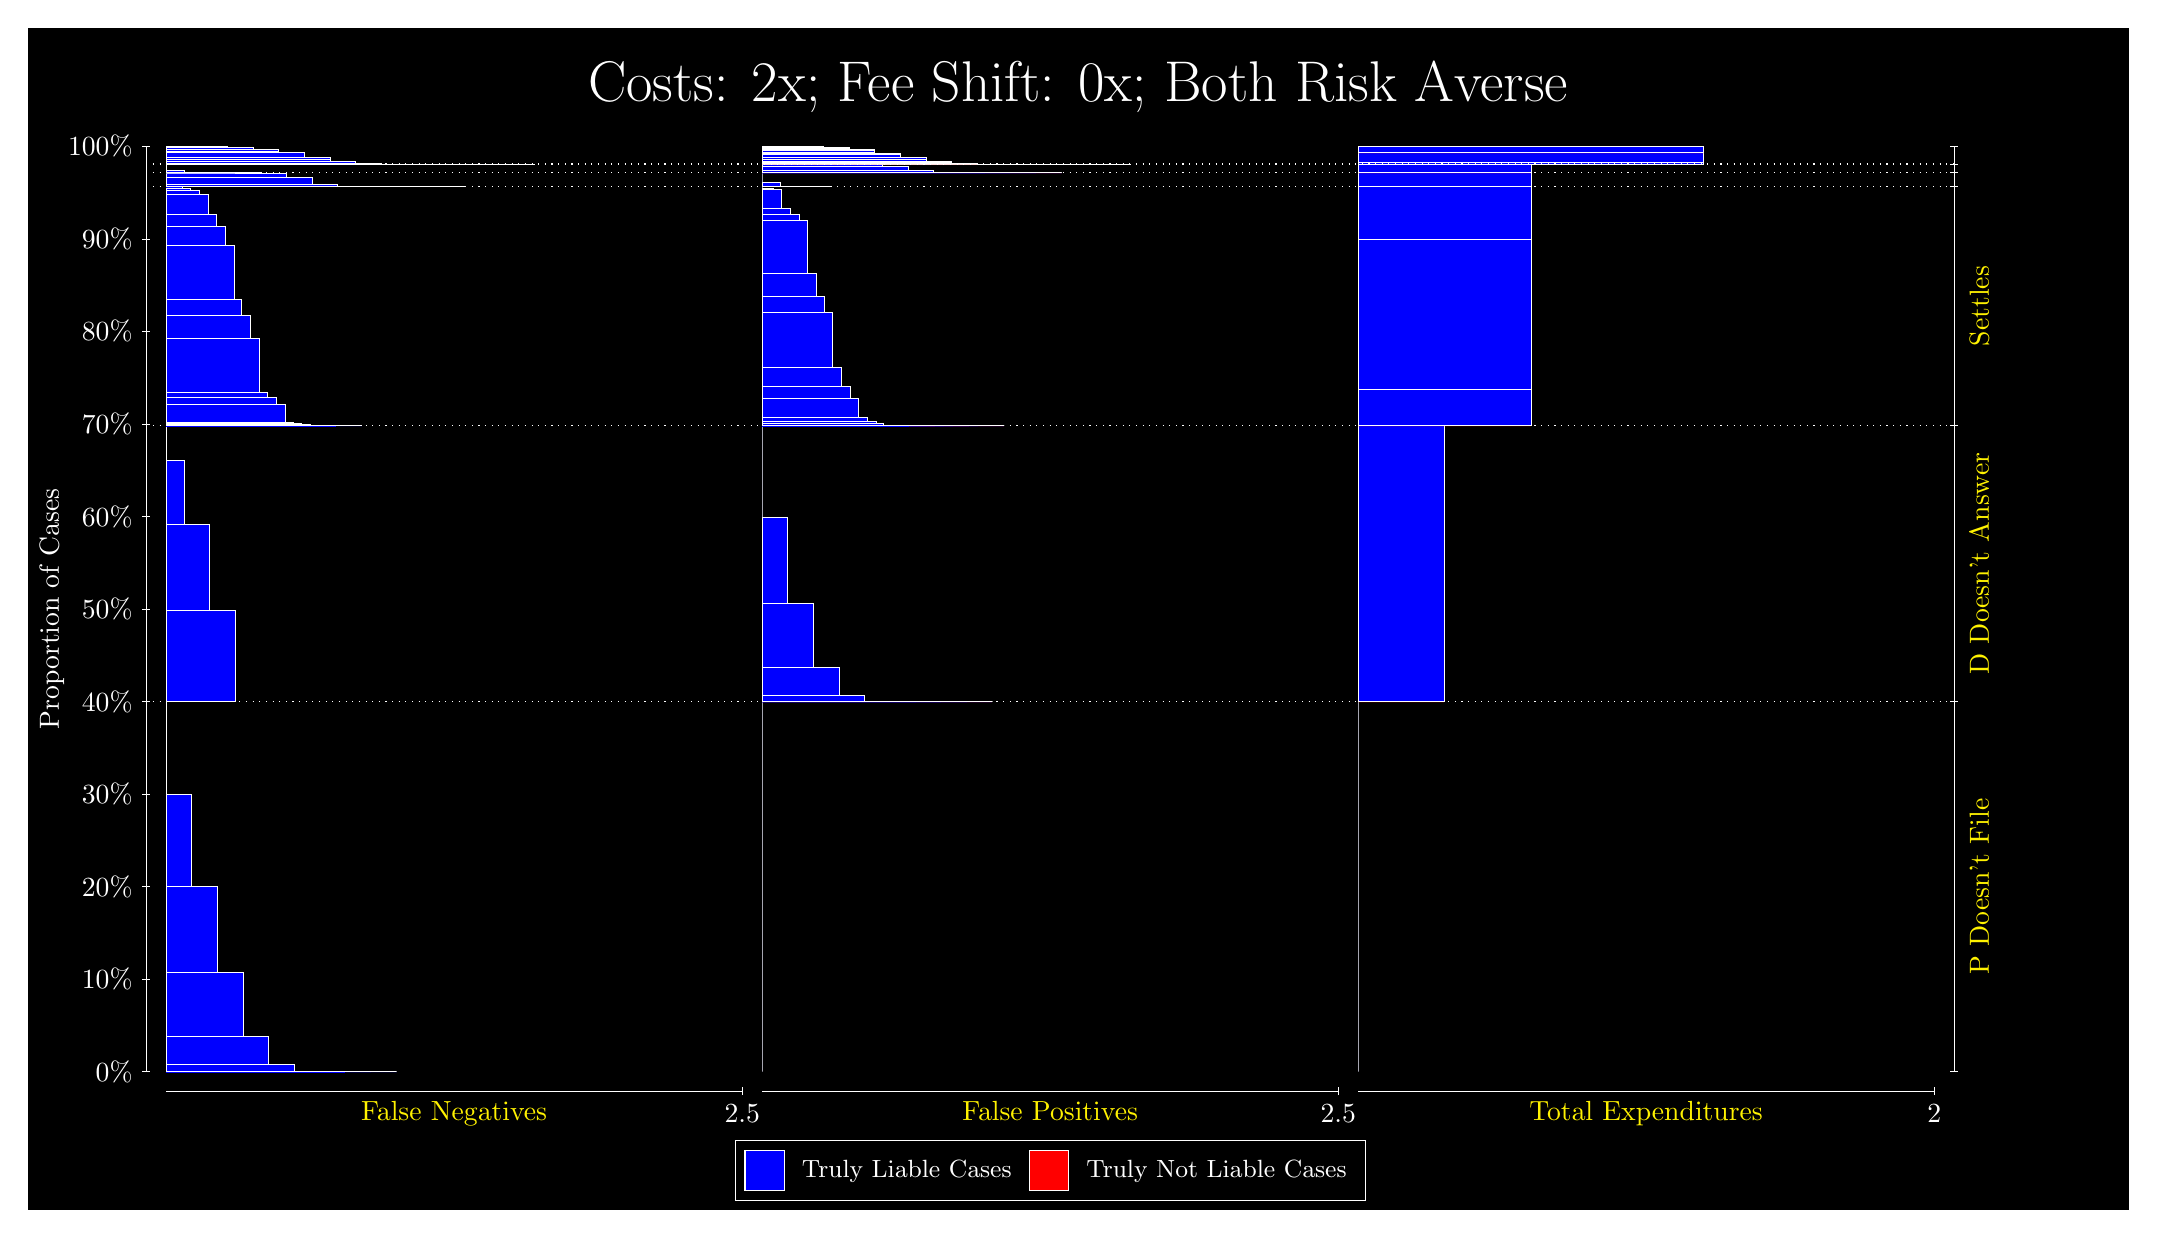
\begin{tikzpicture}
\draw[fill=black] (0,0) rectangle (26.667,15);
\draw[text=white] (0,13.5) rectangle (26.667,15) node[midway] {\huge Costs: 2x; Fee Shift: 0x; Both Risk Averse};
\draw[white, very thin] (1.5,1.75) -- (1.5,13.5);
\node[rotate=90, text=white, anchor=center] at (0.3, 7.625) {Proportion of Cases};
\draw[white, very thin] (1.45,1.75) -- (1.55,1.75);
\node[text=white, anchor=east] at (1.45, 1.75) {0\%};
\draw[white, very thin] (1.45,2.925) -- (1.55,2.925);
\node[text=white, anchor=east] at (1.45, 2.925) {10\%};
\draw[white, very thin] (1.45,4.1) -- (1.55,4.1);
\node[text=white, anchor=east] at (1.45, 4.1) {20\%};
\draw[white, very thin] (1.45,5.275) -- (1.55,5.275);
\node[text=white, anchor=east] at (1.45, 5.275) {30\%};
\draw[white, very thin] (1.45,6.45) -- (1.55,6.45);
\node[text=white, anchor=east] at (1.45, 6.45) {40\%};
\draw[white, very thin] (1.45,7.625) -- (1.55,7.625);
\node[text=white, anchor=east] at (1.45, 7.625) {50\%};
\draw[white, very thin] (1.45,8.8) -- (1.55,8.8);
\node[text=white, anchor=east] at (1.45, 8.8) {60\%};
\draw[white, very thin] (1.45,9.975) -- (1.55,9.975);
\node[text=white, anchor=east] at (1.45, 9.975) {70\%};
\draw[white, very thin] (1.45,11.15) -- (1.55,11.15);
\node[text=white, anchor=east] at (1.45, 11.15) {80\%};
\draw[white, very thin] (1.45,12.325) -- (1.55,12.325);
\node[text=white, anchor=east] at (1.45, 12.325) {90\%};
\draw[white, very thin] (1.45,13.5) -- (1.55,13.5);
\node[text=white, anchor=east] at (1.45, 13.5) {100\%};

\draw[white, very thin] (24.457,1.75) -- (24.457,13.5);
\draw[white, very thin] (24.407,1.75) -- (24.507,1.75);
\node[anchor=west] at (24.407, 1.75) {};
\draw[white, very thin] (24.407,6.4488) -- (24.507,6.4488);
\node[anchor=west] at (24.407, 6.4488) {};
\draw[white, very thin] (24.407,9.9527) -- (24.507,9.9527);
\node[anchor=west] at (24.407, 9.9527) {};
\draw[white, very thin] (24.407,12.991) -- (24.507,12.991);
\node[anchor=west] at (24.407, 12.991) {};
\draw[white, very thin] (24.407,13.167) -- (24.507,13.167);
\node[anchor=west] at (24.407, 13.167) {};
\draw[white, very thin] (24.407,13.276) -- (24.507,13.276);
\node[anchor=west] at (24.407, 13.276) {};
\draw[white, very thin] (24.407,13.5) -- (24.507,13.5);
\node[anchor=west] at (24.407, 13.5) {};

\draw[white, very thin, fill=blue] (1.75,1.75) rectangle (4.6775,1.75);
\draw[white, very thin, fill=blue] (1.75,1.75) rectangle (4.3523,1.75);
\draw[white, very thin, fill=blue] (1.75,1.75) rectangle (4.027,1.7503);
\draw[white, very thin, fill=blue] (1.75,1.7503) rectangle (3.7017,1.7576);
\draw[white, very thin, fill=blue] (1.75,1.7576) rectangle (3.3764,1.8361);
\draw[white, very thin, fill=blue] (1.75,1.8361) rectangle (3.0511,2.1986);
\draw[white, very thin, fill=blue] (1.75,2.1986) rectangle (2.7258,3.011);
\draw[white, very thin, fill=blue] (1.75,3.011) rectangle (2.4006,4.107);
\draw[white, very thin, fill=blue] (1.75,4.107) rectangle (2.0753,5.2742);
\draw[white, very thin, fill=red] (1.75,5.2742) rectangle (1.75,5.2742);
\draw[white, very thin, fill=blue] (1.75,5.2742) rectangle (1.75,6.4488);
\draw[white, very thin, fill=blue] (1.75,6.4488) rectangle (2.6283,7.6133);
\draw[white, very thin, fill=blue] (1.75,7.6133) rectangle (2.303,8.7042);
\draw[white, very thin, fill=blue] (1.75,8.7042) rectangle (1.9777,9.5142);
\draw[white, very thin, fill=red] (1.75,9.5142) rectangle (1.75,9.5142);
\draw[white, very thin, fill=blue] (1.75,9.5142) rectangle (1.75,9.9527);
\draw[white, very thin, fill=blue] (1.75,9.9527) rectangle (4.2384,9.9527);
\draw[white, very thin, fill=blue] (1.75,9.9527) rectangle (3.9131,9.9532);
\draw[white, very thin, fill=blue] (1.75,9.9532) rectangle (3.7993,9.9533);
\draw[white, very thin, fill=blue] (1.75,9.9533) rectangle (3.5878,9.976);
\draw[white, very thin, fill=blue] (1.75,9.976) rectangle (3.474,9.9809);
\draw[white, very thin, fill=blue] (1.75,9.9809) rectangle (3.3602,9.991);
\draw[white, very thin, fill=blue] (1.75,9.991) rectangle (3.2626,10.226);
\draw[white, very thin, fill=blue] (1.75,10.226) rectangle (3.1487,10.308);
\draw[white, very thin, fill=blue] (1.75,10.308) rectangle (3.0349,10.38);
\draw[white, very thin, fill=blue] (1.75,10.38) rectangle (2.9373,11.059);
\draw[white, very thin, fill=blue] (1.75,11.059) rectangle (2.8234,11.351);
\draw[white, very thin, fill=blue] (1.75,11.351) rectangle (2.7096,11.555);
\draw[white, very thin, fill=blue] (1.75,11.555) rectangle (2.612,12.246);
\draw[white, very thin, fill=blue] (1.75,12.246) rectangle (2.4982,12.486);
\draw[white, very thin, fill=blue] (1.75,12.486) rectangle (2.3843,12.641);
\draw[white, very thin, fill=blue] (1.75,12.641) rectangle (2.2867,12.889);
\draw[white, very thin, fill=blue] (1.75,12.889) rectangle (2.1729,12.937);
\draw[white, very thin, fill=blue] (1.75,12.937) rectangle (2.059,12.963);
\draw[white, very thin, fill=blue] (1.75,12.963) rectangle (1.9614,12.987);
\draw[white, very thin, fill=blue] (1.75,12.987) rectangle (1.8476,12.989);
\draw[white, very thin, fill=red] (1.75,12.989) rectangle (1.75,12.989);
\draw[white, very thin, fill=blue] (1.75,12.989) rectangle (1.75,12.991);
\draw[white, very thin, fill=blue] (1.75,12.991) rectangle (5.5558,12.991);
\draw[white, very thin, fill=blue] (1.75,12.991) rectangle (5.2305,12.991);
\draw[white, very thin, fill=blue] (1.75,12.991) rectangle (4.9052,12.991);
\draw[white, very thin, fill=blue] (1.75,12.991) rectangle (4.58,12.991);
\draw[white, very thin, fill=blue] (1.75,12.991) rectangle (4.2547,12.993);
\draw[white, very thin, fill=blue] (1.75,12.993) rectangle (3.9294,13.023);
\draw[white, very thin, fill=blue] (1.75,13.023) rectangle (3.6041,13.11);
\draw[white, very thin, fill=blue] (1.75,13.11) rectangle (3.2788,13.16);
\draw[white, very thin, fill=blue] (1.75,13.16) rectangle (2.9535,13.167);
\draw[white, very thin, fill=blue] (1.75,13.167) rectangle (2.6283,13.167);
\draw[white, very thin, fill=red] (1.75,13.167) rectangle (1.75,13.167);
\draw[white, very thin, fill=blue] (1.75,13.167) rectangle (2.6283,13.167);
\draw[white, very thin, fill=blue] (1.75,13.167) rectangle (2.303,13.171);
\draw[white, very thin, fill=blue] (1.75,13.171) rectangle (1.9777,13.199);
\draw[white, very thin, fill=red] (1.75,13.199) rectangle (1.75,13.199);
\draw[white, very thin, fill=blue] (1.75,13.199) rectangle (1.75,13.276);
\draw[white, very thin, fill=blue] (1.75,13.276) rectangle (6.4341,13.276);
\draw[white, very thin, fill=blue] (1.75,13.276) rectangle (6.1088,13.276);
\draw[white, very thin, fill=blue] (1.75,13.276) rectangle (5.7835,13.276);
\draw[white, very thin, fill=blue] (1.75,13.276) rectangle (5.4582,13.276);
\draw[white, very thin, fill=blue] (1.75,13.276) rectangle (5.1329,13.276);
\draw[white, very thin, fill=blue] (1.75,13.276) rectangle (4.8077,13.277);
\draw[white, very thin, fill=blue] (1.75,13.277) rectangle (4.8077,13.278);
\draw[white, very thin, fill=blue] (1.75,13.278) rectangle (4.4824,13.286);
\draw[white, very thin, fill=blue] (1.75,13.286) rectangle (4.4824,13.286);
\draw[white, very thin, fill=blue] (1.75,13.286) rectangle (4.1571,13.312);
\draw[white, very thin, fill=blue] (1.75,13.312) rectangle (3.8318,13.33);
\draw[white, very thin, fill=blue] (1.75,13.33) rectangle (3.8318,13.36);
\draw[white, very thin, fill=blue] (1.75,13.36) rectangle (3.5065,13.419);
\draw[white, very thin, fill=blue] (1.75,13.419) rectangle (3.1812,13.437);
\draw[white, very thin, fill=blue] (1.75,13.437) rectangle (3.1812,13.443);
\draw[white, very thin, fill=blue] (1.75,13.443) rectangle (3.1812,13.467);
\draw[white, very thin, fill=blue] (1.75,13.467) rectangle (2.856,13.489);
\draw[white, very thin, fill=blue] (1.75,13.489) rectangle (2.856,13.492);
\draw[white, very thin, fill=blue] (1.75,13.492) rectangle (2.5307,13.494);
\draw[white, very thin, fill=blue] (1.75,13.494) rectangle (2.5307,13.495);
\draw[white, very thin, fill=blue] (1.75,13.495) rectangle (2.5307,13.499);
\draw[white, very thin, fill=blue] (1.75,13.499) rectangle (2.2054,13.5);
\draw[white, very thin, fill=blue] (1.75,13.5) rectangle (2.2054,13.5);
\draw[white, very thin, fill=blue] (1.75,13.5) rectangle (1.8801,13.5);
\draw[white, very thin, fill=blue] (1.75,13.5) rectangle (1.8801,13.5);
\draw[white, very thin, fill=red] (1.75,13.5) rectangle (1.75,13.5);
\draw[white, very thin, fill=blue] (1.75,13.5) rectangle (1.75,13.5);
\draw[white, very thin, fill=red] (9.3189,1.75) rectangle (9.3189,1.75);
\draw[white, very thin, fill=blue] (9.3189,1.75) rectangle (9.3189,6.4488);
\draw[white, very thin, fill=red] (9.3189,6.4488) rectangle (12.246,6.4488);
\draw[white, very thin, fill=blue] (9.3189,6.4488) rectangle (12.246,6.4488);
\draw[white, very thin, fill=blue] (9.3189,6.4488) rectangle (11.921,6.4488);
\draw[white, very thin, fill=blue] (9.3189,6.4488) rectangle (11.596,6.4488);
\draw[white, very thin, fill=blue] (9.3189,6.4488) rectangle (11.271,6.4489);
\draw[white, very thin, fill=blue] (9.3189,6.4489) rectangle (10.945,6.454);
\draw[white, very thin, fill=blue] (9.3189,6.454) rectangle (10.62,6.5272);
\draw[white, very thin, fill=blue] (9.3189,6.5272) rectangle (10.295,6.8873);
\draw[white, very thin, fill=blue] (9.3189,6.8873) rectangle (9.9694,7.6973);
\draw[white, very thin, fill=blue] (9.3189,7.6973) rectangle (9.6442,8.7882);
\draw[white, very thin, fill=blue] (9.3189,8.7882) rectangle (9.3189,9.9527);
\draw[white, very thin, fill=red] (9.3189,9.9527) rectangle (12.393,9.9527);
\draw[white, very thin, fill=blue] (9.3189,9.9527) rectangle (12.393,9.9527);
\draw[white, very thin, fill=blue] (9.3189,9.9527) rectangle (12.068,9.9527);
\draw[white, very thin, fill=red] (9.3189,9.9527) rectangle (11.954,9.9527);
\draw[white, very thin, fill=blue] (9.3189,9.9527) rectangle (11.954,9.9527);
\draw[white, very thin, fill=blue] (9.3189,9.9527) rectangle (11.742,9.9527);
\draw[white, very thin, fill=blue] (9.3189,9.9527) rectangle (11.628,9.9527);
\draw[white, very thin, fill=red] (9.3189,9.9527) rectangle (11.515,9.9527);
\draw[white, very thin, fill=blue] (9.3189,9.9527) rectangle (11.515,9.9527);
\draw[white, very thin, fill=blue] (9.3189,9.9527) rectangle (11.417,9.9527);
\draw[white, very thin, fill=blue] (9.3189,9.9527) rectangle (11.303,9.9527);
\draw[white, very thin, fill=blue] (9.3189,9.9527) rectangle (11.189,9.9533);
\draw[white, very thin, fill=blue] (9.3189,9.9533) rectangle (11.092,9.9541);
\draw[white, very thin, fill=blue] (9.3189,9.9541) rectangle (10.978,9.9563);
\draw[white, very thin, fill=blue] (9.3189,9.9563) rectangle (10.864,9.9808);
\draw[white, very thin, fill=blue] (9.3189,9.9808) rectangle (10.766,10.006);
\draw[white, very thin, fill=blue] (9.3189,10.006) rectangle (10.653,10.055);
\draw[white, very thin, fill=blue] (9.3189,10.055) rectangle (10.539,10.302);
\draw[white, very thin, fill=blue] (9.3189,10.302) rectangle (10.441,10.458);
\draw[white, very thin, fill=blue] (9.3189,10.458) rectangle (10.327,10.697);
\draw[white, very thin, fill=blue] (9.3189,10.697) rectangle (10.213,11.389);
\draw[white, very thin, fill=blue] (9.3189,11.389) rectangle (10.116,11.593);
\draw[white, very thin, fill=blue] (9.3189,11.593) rectangle (10.002,11.885);
\draw[white, very thin, fill=blue] (9.3189,11.885) rectangle (9.8881,12.564);
\draw[white, very thin, fill=blue] (9.3189,12.564) rectangle (9.7905,12.635);
\draw[white, very thin, fill=blue] (9.3189,12.635) rectangle (9.6767,12.717);
\draw[white, very thin, fill=blue] (9.3189,12.717) rectangle (9.5628,12.953);
\draw[white, very thin, fill=blue] (9.3189,12.953) rectangle (9.4652,12.963);
\draw[white, very thin, fill=blue] (9.3189,12.963) rectangle (9.3514,12.968);
\draw[white, very thin, fill=blue] (9.3189,12.968) rectangle (9.3189,12.991);
\draw[white, very thin, fill=red] (9.3189,12.991) rectangle (10.197,12.991);
\draw[white, very thin, fill=blue] (9.3189,12.991) rectangle (10.197,12.991);
\draw[white, very thin, fill=blue] (9.3189,12.991) rectangle (9.8718,12.998);
\draw[white, very thin, fill=blue] (9.3189,12.998) rectangle (9.5466,13.048);
\draw[white, very thin, fill=blue] (9.3189,13.048) rectangle (9.3189,13.167);
\draw[white, very thin, fill=red] (9.3189,13.167) rectangle (13.125,13.167);
\draw[white, very thin, fill=blue] (9.3189,13.167) rectangle (13.125,13.167);
\draw[white, very thin, fill=blue] (9.3189,13.167) rectangle (12.799,13.167);
\draw[white, very thin, fill=blue] (9.3189,13.167) rectangle (12.474,13.167);
\draw[white, very thin, fill=blue] (9.3189,13.167) rectangle (12.149,13.167);
\draw[white, very thin, fill=blue] (9.3189,13.167) rectangle (11.824,13.169);
\draw[white, very thin, fill=blue] (9.3189,13.169) rectangle (11.498,13.191);
\draw[white, very thin, fill=blue] (9.3189,13.191) rectangle (11.173,13.244);
\draw[white, very thin, fill=blue] (9.3189,13.244) rectangle (10.848,13.272);
\draw[white, very thin, fill=blue] (9.3189,13.272) rectangle (10.522,13.276);
\draw[white, very thin, fill=blue] (9.3189,13.276) rectangle (10.197,13.276);
\draw[white, very thin, fill=red] (9.3189,13.276) rectangle (14.003,13.276);
\draw[white, very thin, fill=blue] (9.3189,13.276) rectangle (14.003,13.276);
\draw[white, very thin, fill=red] (9.3189,13.276) rectangle (13.678,13.276);
\draw[white, very thin, fill=blue] (9.3189,13.276) rectangle (13.678,13.276);
\draw[white, very thin, fill=red] (9.3189,13.276) rectangle (13.352,13.276);
\draw[white, very thin, fill=blue] (9.3189,13.276) rectangle (13.352,13.276);
\draw[white, very thin, fill=blue] (9.3189,13.276) rectangle (13.027,13.276);
\draw[white, very thin, fill=red] (9.3189,13.276) rectangle (13.027,13.276);
\draw[white, very thin, fill=blue] (9.3189,13.276) rectangle (13.027,13.276);
\draw[white, very thin, fill=blue] (9.3189,13.276) rectangle (12.702,13.276);
\draw[white, very thin, fill=red] (9.3189,13.276) rectangle (12.702,13.276);
\draw[white, very thin, fill=blue] (9.3189,13.276) rectangle (12.702,13.276);
\draw[white, very thin, fill=blue] (9.3189,13.276) rectangle (12.377,13.277);
\draw[white, very thin, fill=red] (9.3189,13.277) rectangle (12.377,13.277);
\draw[white, very thin, fill=blue] (9.3189,13.277) rectangle (12.377,13.277);
\draw[white, very thin, fill=blue] (9.3189,13.277) rectangle (12.051,13.28);
\draw[white, very thin, fill=red] (9.3189,13.28) rectangle (12.051,13.28);
\draw[white, very thin, fill=blue] (9.3189,13.28) rectangle (12.051,13.284);
\draw[white, very thin, fill=blue] (9.3189,13.284) rectangle (12.051,13.285);
\draw[white, very thin, fill=blue] (9.3189,13.285) rectangle (12.051,13.285);
\draw[white, very thin, fill=blue] (9.3189,13.285) rectangle (11.726,13.296);
\draw[white, very thin, fill=red] (9.3189,13.296) rectangle (11.726,13.296);
\draw[white, very thin, fill=blue] (9.3189,13.296) rectangle (11.726,13.309);
\draw[white, very thin, fill=blue] (9.3189,13.309) rectangle (11.726,13.309);
\draw[white, very thin, fill=blue] (9.3189,13.309) rectangle (11.401,13.31);
\draw[white, very thin, fill=blue] (9.3189,13.31) rectangle (11.401,13.333);
\draw[white, very thin, fill=red] (9.3189,13.333) rectangle (11.401,13.333);
\draw[white, very thin, fill=blue] (9.3189,13.333) rectangle (11.401,13.357);
\draw[white, very thin, fill=blue] (9.3189,13.357) rectangle (11.075,13.365);
\draw[white, very thin, fill=red] (9.3189,13.365) rectangle (11.075,13.365);
\draw[white, very thin, fill=blue] (9.3189,13.365) rectangle (11.075,13.393);
\draw[white, very thin, fill=blue] (9.3189,13.393) rectangle (11.075,13.417);
\draw[white, very thin, fill=blue] (9.3189,13.417) rectangle (10.75,13.425);
\draw[white, very thin, fill=blue] (9.3189,13.425) rectangle (10.75,13.43);
\draw[white, very thin, fill=blue] (9.3189,13.43) rectangle (10.75,13.453);
\draw[white, very thin, fill=blue] (9.3189,13.453) rectangle (10.75,13.465);
\draw[white, very thin, fill=blue] (9.3189,13.465) rectangle (10.425,13.476);
\draw[white, very thin, fill=blue] (9.3189,13.476) rectangle (10.425,13.478);
\draw[white, very thin, fill=blue] (9.3189,13.478) rectangle (10.425,13.49);
\draw[white, very thin, fill=blue] (9.3189,13.49) rectangle (10.1,13.492);
\draw[white, very thin, fill=blue] (9.3189,13.492) rectangle (10.1,13.493);
\draw[white, very thin, fill=blue] (9.3189,13.493) rectangle (10.1,13.497);
\draw[white, very thin, fill=blue] (9.3189,13.497) rectangle (10.1,13.498);
\draw[white, very thin, fill=blue] (9.3189,13.498) rectangle (9.7743,13.499);
\draw[white, very thin, fill=blue] (9.3189,13.499) rectangle (9.7743,13.5);
\draw[white, very thin, fill=blue] (9.3189,13.5) rectangle (9.449,13.5);
\draw[white, very thin, fill=blue] (9.3189,13.5) rectangle (9.449,13.5);
\draw[white, very thin, fill=blue] (9.3189,13.5) rectangle (9.449,13.5);
\draw[white, very thin, fill=blue] (9.3189,13.5) rectangle (9.3189,13.5);
\draw[white, very thin, fill=red] (16.888,1.75) rectangle (16.888,1.75);
\draw[white, very thin, fill=blue] (16.888,1.75) rectangle (16.888,6.4488);
\draw[white, very thin, fill=red] (16.888,6.4488) rectangle (17.986,6.4488);
\draw[white, very thin, fill=blue] (16.888,6.4488) rectangle (17.986,9.9527);
\draw[white, very thin, fill=red] (16.888,9.9527) rectangle (19.083,9.9527);
\draw[white, very thin, fill=blue] (16.888,9.9527) rectangle (19.083,10.419);
\draw[white, very thin, fill=red] (16.888,10.419) rectangle (19.083,10.419);
\draw[white, very thin, fill=blue] (16.888,10.419) rectangle (19.083,12.321);
\draw[white, very thin, fill=red] (16.888,12.321) rectangle (19.083,12.321);
\draw[white, very thin, fill=blue] (16.888,12.321) rectangle (19.083,12.991);
\draw[white, very thin, fill=red] (16.888,12.991) rectangle (19.083,12.991);
\draw[white, very thin, fill=blue] (16.888,12.991) rectangle (19.083,13.167);
\draw[white, very thin, fill=red] (16.888,13.167) rectangle (19.083,13.167);
\draw[white, very thin, fill=blue] (16.888,13.167) rectangle (19.083,13.276);
\draw[white, very thin, fill=red] (16.888,13.276) rectangle (21.279,13.276);
\draw[white, very thin, fill=blue] (16.888,13.276) rectangle (21.279,13.302);
\draw[white, very thin, fill=red] (16.888,13.302) rectangle (21.279,13.302);
\draw[white, very thin, fill=blue] (16.888,13.302) rectangle (21.279,13.421);
\draw[white, very thin, fill=red] (16.888,13.421) rectangle (21.279,13.421);
\draw[white, very thin, fill=blue] (16.888,13.421) rectangle (21.279,13.5);
\draw[white, dotted] (1.5,6.4488) -- (24.457,6.4488);
\draw[white, dotted] (1.5,9.9527) -- (24.457,9.9527);
\draw[white, dotted] (1.5,12.991) -- (24.457,12.991);
\draw[white, dotted] (1.5,13.167) -- (24.457,13.167);
\draw[white, dotted] (1.5,13.276) -- (24.457,13.276);
\draw[white, very thin] (1.75,1.5) -- (9.0689,1.5);
\node[text=yellow, anchor=north] at (5.4094, 1.5) {False Negatives};
\draw[white, very thin] (9.0689,1.45) -- (9.0689,1.55);
\node[text=white, anchor=north] at (9.0689, 1.45) {2.5};

\draw[white, very thin] (9.3189,1.5) -- (16.638,1.5);
\node[text=yellow, anchor=north] at (12.978, 1.5) {False Positives};
\draw[white, very thin] (16.638,1.45) -- (16.638,1.55);
\node[text=white, anchor=north] at (16.638, 1.45) {2.5};

\draw[white, very thin] (16.888,1.5) -- (24.207,1.5);
\node[text=yellow, anchor=north] at (20.547, 1.5) {Total Expenditures};
\draw[white, very thin] (24.207,1.45) -- (24.207,1.55);
\node[text=white, anchor=north] at (24.207, 1.45) {2};

\node[text=yellow, centered, rotate=90] at (24.777, 4.0994) {P Doesn't File};
\node[text=yellow, centered, rotate=90] at (24.777, 8.2007) {D Doesn't Answer};
\node[text=yellow, centered, rotate=90] at (24.777, 11.472) {Settles};




\draw (12.978300999999998,1.5) node[draw=none] (baseCoordinate) {};
\begin{scope}[align=center]
        \matrix[scale=0.5, draw=white, below=0.5cm of baseCoordinate, nodes={draw}, column sep=0.1cm]{
            \node[rectangle, draw, minimum width=0.5cm, minimum height=0.5cm, fill=blue] {}; &
            \node[draw=none, font=\small, text=white] (B) {Truly Liable Cases}; &
            \node[rectangle, draw, minimum width=0.5cm, minimum height=0.5cm, fill=red] {}; &
            \node[draw=none, font=\small, text=white] (B) {Truly Not Liable Cases}; \\
            };
\end{scope}

\end{tikzpicture}
\end{document}